% ============================================================
%  Springer LNCS article -- open in Overleaf
%  Compiler: pdfLaTeX   |   Bibliography: BibTeX (splncs04)
% ============================================================
\documentclass[runningheads]{llncs}

\usepackage[T1]{fontenc}
\usepackage{graphicx}
\usepackage{amsmath,amssymb}
\usepackage{booktabs}
\usepackage{tabularx}
\usepackage{tikz}
\usetikzlibrary{arrows.meta,positioning}
\usepackage{algorithm}
\usepackage{algpseudocode}
\usepackage{hyperref}
\renewcommand\UrlFont{\color{blue}\rmfamily}

\begin{document}

\title{Securing Electric Vehicle Charging Infrastructure: Analysis of Existing Security Tools and a Layered Protocol-Aware Approach}
\titlerunning{Securing EV Charging Infrastructure}

% ---- EDIT YOUR DETAILS HERE ----
\author{Your Name}
\authorrunning{Your Name}
\institute{Department of Computer Science and Engineering\\
Your College Name\\
India}
% --------------------------------

\maketitle

\begin{abstract}
Electric Vehicle (EV) charging stations are becoming part of the critical energy infrastructure. A modern charging station is a networked computer that communicates with the vehicle using ISO~15118, with a cloud management system using the Open Charge Point Protocol (OCPP), and indirectly with payment systems and the power grid. These connections introduce security problems such as publicly exposed management interfaces, unencrypted protocol messages, forged meter readings, unsigned firmware updates and wireless disruption of charging sessions.

This paper first verifies these problems by mapping them onto the phases of an attack: reconnaissance, scanning, gaining access, maintaining access and covering tracks. It then analyses existing security tools such as Nmap, Shodan, Nessus, Wireshark, Snort and SIEM platforms, and shows that they are largely protocol-unaware for this domain. Finally, a layered approach called ChargeShield is proposed. It combines elliptic-curve based mutual authentication, OCPP-aware message inspection, unsupervised anomaly detection on charging data, and a zero-trust policy layer. A Python prototype was evaluated on ten simulated days of synthetic OCPP traffic from twenty chargers. In this evaluation, the protocol-aware layer detected all forged messages without false alarms, while a syntax-only baseline detected one quarter of them. The behavioural layer detected all simulated misuse windows with a false positive rate of about 0.5\%.

\keywords{EV Charging Security \and OCPP \and ISO 15118 \and Public-Key Cryptography \and Intrusion Detection \and Anomaly Detection \and Zero Trust}
\end{abstract}

% ============================================================
\section{Introduction}
% ============================================================
The number of electric vehicles is increasing rapidly, and with it the number of public and private charging stations. Unlike a fuel pump, a charging station, also called Electric Vehicle Supply Equipment (EVSE), is a small computer. It runs an embedded operating system, stores cryptographic credentials, communicates over the internet, processes payments and controls a high-power electrical connection.

A charging station communicates with three main parties. It talks to the vehicle using ISO~15118~\cite{iso15118}, to the operator's Charging Station Management System (CSMS) using OCPP~\cite{ocpp201}, and, through the CSMS, to payment providers and the power grid. A weakness in any of these links can lead to energy theft, billing fraud, theft of payment data, denial of charging, and, in the worst case, coordinated switching of many chargers that can disturb the local power grid~\cite{johnson2022review,antoun2020detailed}.

The basic security goals of Confidentiality, Integrity and Availability (CIA), together with authentication and non-repudiation~\cite{stallings2017}, apply directly to this domain. Confidentiality protects driver identities and payment tokens. Integrity protects meter values, tariffs and firmware. Availability ensures that drivers can charge their vehicles. Authentication ensures that only legitimate chargers, vehicles and servers take part in the system.

Many security tools are already available on the market, including port scanners, vulnerability scanners, packet analysers, intrusion detection systems and log correlation platforms. These tools work well in traditional IT networks, but they generally do not understand the meaning of OCPP or ISO~15118 messages. A forged meter reading, for example, is a perfectly well-formed message and is therefore not detected by a signature-based system.

This paper therefore focuses on three objectives: first, to verify the security problems of EV charging infrastructure; second, to analyse existing security tools and identify their limitations in this domain; and third, to propose a layered approach that can overcome these limitations.

% ============================================================
\section{Background and Related Work}
% ============================================================
\subsection{EV Charging Architecture}
Figure~\ref{fig:arch} shows the main components of the charging ecosystem. For DC fast charging under the Combined Charging System (CCS), the vehicle and charger exchange ISO~15118 messages over power-line communication (PLC) in the charging cable. The charger connects to the CSMS over cellular or Ethernet networks using OCPP, which sends JSON messages over WebSockets. Typical OCPP messages include \texttt{BootNotification}, \texttt{Authorize}, \texttt{StartTransaction}, \texttt{MeterValues}, \texttt{RemoteStartTransaction} and \texttt{UpdateFirmware}.

\begin{figure}[t]
\centering
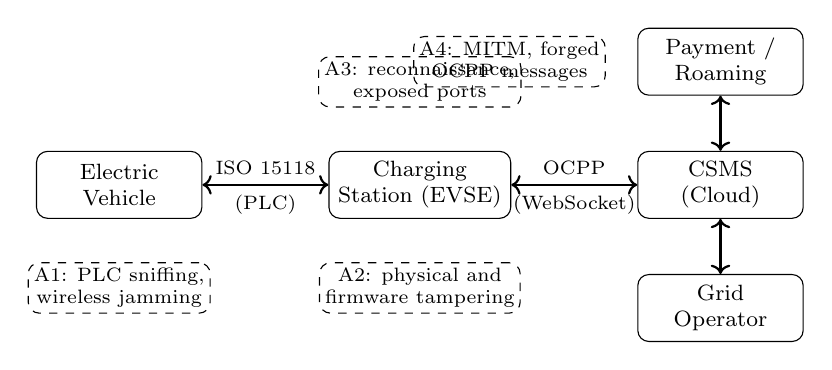
\begin{tikzpicture}[
  box/.style={draw, rounded corners, minimum width=2.1cm, minimum height=0.85cm, align=center, font=\footnotesize},
  atk/.style={draw, dashed, rounded corners, font=\scriptsize, align=center, inner sep=2pt},
  arr/.style={-{Latex[length=2mm]}, thick},
  lbl/.style={font=\scriptsize, midway, above}
]
\node[box] (ev) {Electric\\Vehicle};
\node[box, right=1.6cm of ev] (evse) {Charging\\Station (EVSE)};
\node[box, right=1.6cm of evse] (csms) {CSMS\\(Cloud)};
\node[box, above=0.7cm of csms] (pay) {Payment /\\Roaming};
\node[box, below=0.7cm of csms] (dso) {Grid\\Operator};
\draw[arr, <->] (ev) -- node[lbl]{ISO 15118} node[font=\scriptsize, midway, below]{(PLC)} (evse);
\draw[arr, <->] (evse) -- node[lbl]{OCPP} node[font=\scriptsize, midway, below]{(WebSocket)} (csms);
\draw[arr, <->] (csms) -- (pay);
\draw[arr, <->] (csms) -- (dso);
\node[atk, below=0.55cm of ev] {A1: PLC sniffing,\\wireless jamming};
\node[atk, below=0.55cm of evse] {A2: physical and\\firmware tampering};
\node[atk, above=0.55cm of evse] {A3: reconnaissance,\\exposed ports};
\node[atk, left=0.4cm of pay] {A4: MITM, forged\\OCPP messages};
\end{tikzpicture}
\caption{EV charging architecture and main attack surfaces (A1--A4)}
\label{fig:arch}
\end{figure}

OCPP~2.0.1 defines three security profiles~\cite{ocpp201}: Profile~1 uses HTTP Basic authentication without TLS; Profile~2 uses TLS with Basic authentication; and Profile~3 uses TLS with mutual certificate authentication. ISO~15118 adds \emph{Plug \& Charge}, in which the vehicle authenticates automatically using an X.509 contract certificate issued under a Vehicle-to-Grid (V2G) public-key infrastructure~\cite{iso15118}. In practice, many installed chargers still use the older OCPP~1.6 or Profile~1 because certificate management is difficult.

\subsection{Related Work}
Alcaraz et al.~\cite{alcaraz2017ocpp} analysed OCPP and identified man-in-the-middle, impersonation and data manipulation threats. They showed that older OCPP versions did not require transport security.

Antoun et al.~\cite{antoun2020detailed} assessed the complete charging ecosystem, including vehicles, chargers, management systems and mobile applications, and showed that a weakness in one component can affect the whole chain.

Johnson et al.~\cite{johnson2022review} reviewed publicly reported charger vulnerabilities and discussed their possible impact on the power grid. Gottumukkala et al.~\cite{gottumukkala2019cyber} performed practical security tests on commercial charging stations and reported weak authentication and unnecessary open services.

Baker and Martinovic~\cite{baker2019losing} showed that the PLC signal used in CCS charging can be eavesdropped wirelessly. K\"ohler et al.~\cite{kohler2023brokenwire} presented \emph{Brokenwire}, an attack that interrupts CCS charging sessions from a distance using low-cost radio equipment.

For intrusion detection, signature-based tools such as Snort~\cite{roesch1999snort} and monitoring tools such as Bro/Zeek~\cite{paxson1999bro} are widely used. Anomaly detection methods such as Isolation Forest~\cite{liu2008isolation} and autoencoder ensembles such as Kitsune~\cite{mirsky2018kitsune} can identify previously unseen attacks. Sommer and Paxson~\cite{sommer2010outside}, however, noted that machine learning detectors can produce many false alarms when they lack domain knowledge.

Existing research shows that EV charging has real and documented security problems, but it gives less attention to how existing security tools can be extended or combined to address them.

% ============================================================
\section{Verified Security Problems in EV Charging}
% ============================================================
To verify the problems in a structured way, they are mapped onto the five phases of an attack used in ethical hacking.

\subsection{Reconnaissance}
Public charging maps publish the location, vendor and model of many stations. Internet-wide search engines such as Shodan~\cite{matherly2015shodan}, which rely on fast scanners like ZMap~\cite{durumeric2013zmap}, index exposed web panels, remote login services and OCPP endpoints. An attacker can therefore build a list of targets without sending any packet to them.

\subsection{Scanning and Enumeration}
Active scanning with Nmap~\cite{lyon2009nmap} can reveal open ports such as 22 (SSH), 23 (Telnet), 80/443 (web interface), 502 (Modbus) and the OCPP port. Enumeration can then identify default credentials and outdated software versions~\cite{gottumukkala2019cyber}.

\subsection{Gaining Access}
When OCPP runs without TLS, the server identifies a charger only by its \texttt{ChargePointId} and a static password. An attacker who learns these values can impersonate the charger and send false \texttt{MeterValues}, or impersonate the server and send commands such as \texttt{RemoteStartTransaction} or \texttt{UpdateFirmware}~\cite{alcaraz2017ocpp}. Other entry points include PLC eavesdropping~\cite{baker2019losing}, exposed USB or debug ports, and hard-coded keys.

\subsection{Maintaining Access}
An attacker can install modified firmware that survives reboots. Because many chargers of the same model run identical firmware, one successful exploit can be repeated across a large number of stations and used for coordinated load switching~\cite{johnson2022review}.

\subsection{Covering Tracks and Denial of Service}
Chargers usually keep limited local logs, and these logs are often not forwarded to a central system. In addition, wireless attacks such as Brokenwire~\cite{kohler2023brokenwire} can stop charging without leaving any trace in network logs.

Table~\ref{tab:problems} summarises the verified problems.

\begin{table}[t]
\centering
\caption{Verified security problems in EV charging infrastructure}
\label{tab:problems}
\footnotesize
\begin{tabularx}{\textwidth}{@{}l X l@{}}
\toprule
\textbf{ID} & \textbf{Problem} & \textbf{Security goal affected}\\
\midrule
P1 & Station details and exposed services are publicly indexed & Confidentiality \\
P2 & Default credentials and unnecessary open ports & Authentication \\
P3 & OCPP without TLS; spoofed charger or server & Integrity, Authentication\\
P4 & Forged meter values (billing fraud) & Integrity \\
P5 & Unsigned or unverified firmware updates & Integrity \\
P6 & Weak key management: hard-coded keys, no revocation & Authentication \\
P7 & PLC eavesdropping and wireless session disruption & Confidentiality, Availability \\
P8 & Coordinated load switching using many chargers & Availability \\
P9 & Insufficient logging and central monitoring & Non-repudiation \\
\bottomrule
\end{tabularx}
\end{table}

% ============================================================
\section{Analysis of Existing Security Tools}
% ============================================================
Several widely used tools can be applied to charging networks. Each provides useful protection, but each also has limitations in this domain, as summarised in Table~\ref{tab:tools}.

\begin{table}[t]
\centering
\caption{Comparison of existing security tools for EV charging}
\label{tab:tools}
\footnotesize
\begin{tabularx}{\textwidth}{@{}l l X@{}}
\toprule
\textbf{Tool} & \textbf{Main Method} & \textbf{Main Limitation}\\
\midrule
Nmap & Port and service scanning & No knowledge of OCPP or of which security profile is in use\\
Shodan & Internet-wide search & Mostly useful to attackers; gives defenders only a snapshot\\
Nessus / OpenVAS & Known vulnerability checks & Generic CVE checks; no tests for insecure OCPP settings\\
Wireshark & Manual packet analysis & Manual and offline; cannot inspect encrypted traffic\\
Snort / Suricata & Signature-based detection & Matches patterns, not meaning; misses unknown attacks\\
Zeek & Scriptable monitoring & No built-in OCPP analyser\\
SIEM & Log correlation & Depends on logs that chargers rarely provide\\
Generic PKI & Certificate issuing & Not designed for V2G certificates or large device fleets\\
\bottomrule
\end{tabularx}
\end{table}

From this analysis, four main gaps are identified:
\begin{enumerate}
  \item \textbf{G1, protocol blindness:} the tools do not understand OCPP and ISO~15118 messages.
  \item \textbf{G2, weak identity:} certificate management for thousands of chargers is not supported.
  \item \textbf{G3, unknown attacks:} signature-based detection cannot identify new or gradual attacks.
  \item \textbf{G4, implicit trust:} devices inside the operator network are trusted by default.
\end{enumerate}

% ============================================================
\section{Proposed Approach: ChargeShield}
% ============================================================
The proposed approach, ChargeShield, adds four layers of protection, as shown in Fig.~\ref{fig:chargeshield}. The lower layers prevent attacks, while the upper layers detect attacks and respond to them.

\begin{figure}[t]
\centering
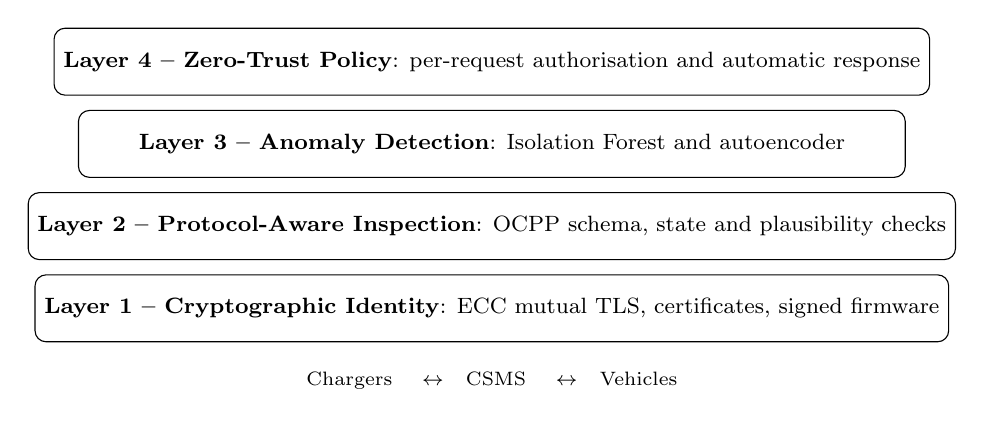
\begin{tikzpicture}[
  layer/.style={draw, rounded corners, minimum width=10.5cm, minimum height=0.85cm, align=center, font=\footnotesize},
  node distance=0.18cm
]
\node[layer] (l4) {\textbf{Layer 4 -- Zero-Trust Policy}: per-request authorisation and automatic response};
\node[layer, below=of l4] (l3) {\textbf{Layer 3 -- Anomaly Detection}: Isolation Forest and autoencoder};
\node[layer, below=of l3] (l2) {\textbf{Layer 2 -- Protocol-Aware Inspection}: OCPP schema, state and plausibility checks};
\node[layer, below=of l2] (l1) {\textbf{Layer 1 -- Cryptographic Identity}: ECC mutual TLS, certificates, signed firmware};
\node[font=\scriptsize, below=0.25cm of l1] {Chargers \quad$\leftrightarrow$\quad CSMS \quad$\leftrightarrow$\quad Vehicles};
\end{tikzpicture}
\caption{Proposed layered architecture of ChargeShield}
\label{fig:chargeshield}
\end{figure}

\subsection{Layer 1: Cryptographic Identity}
Each charger receives a unique key pair generated inside a secure hardware element, so the private key cannot be copied. Communication uses OCPP Security Profile~3, which is TLS~1.3~\cite{rfc8446} with mutual certificate authentication.

Elliptic-curve cryptography (ECC)~\cite{koblitz1987elliptic} is preferred over RSA~\cite{rivest1978method} because it provides similar security with much smaller keys, which is important for embedded devices. Keys are exchanged using ephemeral elliptic-curve Diffie--Hellman~\cite{diffie1976new}. If $G$ is a public base point, the charger chooses a secret $a$ and sends $A = aG$, and the server chooses a secret $b$ and sends $B = bG$. Both sides compute the shared secret
\begin{equation}
K = aB = bA = abG.
\end{equation}
Because $a$ and $b$ are deleted after the session, past sessions remain protected even if a long-term key is stolen later. This property is called forward secrecy.

Certificates are short-lived and renewed automatically using the OCPP \texttt{SignCertificate} message, and their revocation status is checked using OCSP. Firmware images are signed by the vendor:
\begin{equation}
\sigma = \mathrm{Sign}_{sk_v}\big(H(\mathit{firmware})\big),
\end{equation}
where $H$ is SHA-256. The charger verifies $\sigma$ before installing or running the firmware.

\subsection{Layer 2: Protocol-Aware Inspection}
Because TLS encrypts the traffic, a network IDS cannot read OCPP messages. The inspection engine is therefore placed at the entrance of the CSMS as a WebSocket proxy, where messages are already decrypted. It performs three checks:
\begin{itemize}
  \item \textbf{Schema check:} each message must match the official OCPP JSON schema.
  \item \textbf{State check:} messages must follow the correct order, for example \emph{Available}, \emph{Preparing}, \emph{Charging}, \emph{Finishing}.
  \item \textbf{Plausibility check:} meter values must follow physical limits.
\end{itemize}
The procedure is shown in Algorithm~\ref{alg:dpi}.

\begin{algorithm}[t]
\caption{Inspection of an incoming OCPP message}
\label{alg:dpi}
\footnotesize
\begin{algorithmic}[1]
\Require message $m$ from charger $c$, state table $S$, rated power $P_{\max}(c)$
\If{$m$ does not match the OCPP schema} \State \Return \textsc{Block} \EndIf
\If{$m.\mathit{action}$ is not allowed in state $S[c]$} \State \Return \textsc{Alert} \EndIf
\If{$m.\mathit{action} = \texttt{MeterValues}$}
  \State $\Delta E \gets m.E - S[c].E_{\mathrm{last}}$, \quad $\Delta t \gets m.t - S[c].t_{\mathrm{last}}$
  \If{$\Delta E < 0$ \textbf{or} $\Delta E / \Delta t > P_{\max}(c)$} \State \Return \textsc{Alert} \EndIf
\EndIf
\State update $S[c]$ and send features to Layer~3
\State \Return \textsc{Forward}
\end{algorithmic}
\end{algorithm}

\subsection{Layer 3: Anomaly Detection}
Rule checks can only detect known types of misuse. To detect unknown attacks, unsupervised anomaly detection is used. This is suitable because labelled attack data for EV charging is rarely available. The models are described in Section~\ref{sec:models}.

\subsection{Layer 4: Zero-Trust Policy}
Following NIST SP~800-207~\cite{nist800207}, no device is trusted because of its network location. Every request is authorised using the identity of the sender, the requested action and the current risk score from Layers~2 and~3. High-impact commands such as \texttt{UpdateFirmware}, \texttt{Reset} or fleet-wide \texttt{SetChargingProfile} require approval by two operators. Each charger can only reach the CSMS endpoint. When an attack is detected, the system can raise an alert, revoke the charger's certificate, or switch the charger to a safe local mode.

% ============================================================
\section{Detection Models}\label{sec:models}
% ============================================================
Each charger is described in each time window by a feature vector $x$. The features include the message rate for each message type, the time between messages, the session duration, the energy delivered, the number of failed authentication attempts and the number of configuration changes.

\subsection{Plausibility Rules}
For two consecutive meter readings $E_t$ and $E_{t-1}$, the average power is
\begin{equation}
P_t = \frac{E_t - E_{t-1}}{\Delta t}.
\end{equation}
A reading is flagged if $E_t < E_{t-1}$ or if $P_t > P_{\max}$, the rated power of the connector.

\subsection{Isolation Forest}
Isolation Forest~\cite{liu2008isolation} builds random trees that split the data using random features and values. Unusual points are separated after fewer splits. The anomaly score is
\begin{equation}
s(x, n) = 2^{-\frac{E[h(x)]}{c(n)}},
\end{equation}
where $h(x)$ is the path length of $x$ and $c(n)$ is the average path length for $n$ samples. A score close to $1$ indicates an anomaly.

\subsection{Autoencoder}
An autoencoder is a neural network that learns to reconstruct normal input. Following the idea of Kitsune~\cite{mirsky2018kitsune}, the reconstruction error
\begin{equation}
e(x) = \lVert x - \hat{x} \rVert_2
\end{equation}
is used as an anomaly score, where $\hat{x}$ is the reconstructed input. A high error means that the behaviour is different from normal.

\subsection{Robust Range Check}
Isolation Forest only splits within the range of values seen during training, so a value far outside that range is not isolated faster than the most extreme normal sample. To cover this case, each feature $j$ is also compared with its normal median $\mathrm{med}_j$ using a robust z-score based on the median absolute deviation (MAD):
\begin{equation}
z_j(x) = \frac{x_j - \mathrm{med}_j}{\max(1.4826 \cdot \mathrm{MAD}_j,\ 1)}.
\end{equation}
A window is flagged if $z_j(x) > 6$ for any feature, or if the Isolation Forest score is below the 0.5th percentile of the training scores.

\subsection{Fleet-Level Correlation}
Some attacks only become visible when many chargers are observed together. If a large number of chargers receive sudden \texttt{SetChargingProfile} changes within a short time, the system raises an alert for a possible coordinated grid attack.

% ============================================================
\section{Performance Evaluation}
% ============================================================
The approach should be evaluated using standard detection metrics. Here TP is the number of attacks correctly detected, TN the number of normal events correctly accepted, FP the number of normal events wrongly flagged, and FN the number of attacks missed.

\subsection{Detection Rate (Recall)}
\begin{equation}
\mathit{Recall} = \frac{TP}{TP + FN}.
\end{equation}

\subsection{Precision}
\begin{equation}
\mathit{Precision} = \frac{TP}{TP + FP}.
\end{equation}

\subsection{False Positive Rate}
\begin{equation}
\mathit{FPR} = \frac{FP}{FP + TN}.
\end{equation}

\subsection{F1-Score}
\begin{equation}
F1 = 2 \times \frac{\mathit{Precision} \times \mathit{Recall}}{\mathit{Precision} + \mathit{Recall}}.
\end{equation}

\subsection{Added Latency}
Because Layer~2 inspects messages inline, the additional delay per message must also be measured. It should stay well below the OCPP response timeout of several seconds.

For EV charging, a high recall is important because a missed attack can cause financial loss or grid problems. A low false positive rate is equally important because wrongly blocking a charger prevents drivers from charging.

% ============================================================
\section{Experimental Design}
% ============================================================
A prototype of Layers~1--3, the fleet correlation and a simple Layer~4 response policy was implemented in Python using scikit-learn and the \texttt{cryptography} library. The source code is available at \url{https://github.com/Dxrshpreet/ev-charging-security-article}. The evaluation followed this workflow:
\begin{enumerate}
  \item Generate one day of normal OCPP traffic from 20 simulated chargers (22~kW and 50~kW) as training data.
  \item Train the Isolation Forest and the robust range check on normal traffic only.
  \item Generate a separate test day and inject attacks with ground-truth labels: 20 forged messages (5 malformed, 5 spoofed transactions, 5 meter rollbacks, 5 physically impossible readings); 6 misuse windows (2 RFID card brute-force, 2 message floods, 2 configuration tampering); and 1 fleet-wide \texttt{SetChargingProfile} attack on 15 chargers.
  \item Run the same traffic through a syntax-only baseline, which accepts any well-formed message, as a stand-in for a protocol-unaware detector.
  \item Calculate recall, precision, false positive rate, F1-score and inspection time per message.
  \item Repeat for ten simulated days (random seeds 1--10) and report the mean.
\end{enumerate}
Each test day contains about 20{,}000 messages and 480 charger-hour windows. Table~\ref{tab:results} shows the results.

\begin{table}[t]
\centering
\caption{Performance of the prototype on synthetic traffic (mean of 10 simulated days)}
\label{tab:results}
\footnotesize
\begin{tabular}{@{}l c c c c c@{}}
\toprule
\textbf{Approach} & \textbf{Recall} & \textbf{Precision} & \textbf{FPR} & \textbf{F1} & \textbf{Time/msg}\\
\midrule
\multicolumn{6}{@{}l}{\emph{Per message (forged OCPP messages)}}\\
Syntax-only baseline & 0.25 & 1.00 & 0.0000 & 0.40 & 8.5\,$\mu$s \\
Layer 2 inspection & 1.00 & 1.00 & 0.0000 & 1.00 & 19.5\,$\mu$s \\
\midrule
\multicolumn{6}{@{}l}{\emph{Per charger-hour window (behavioural misuse)}}\\
Isolation Forest only & 0.15 & 0.42 & 0.0053 & 0.21 & -- \\
Robust range check only & 1.00 & 1.00 & 0.0000 & 1.00 & -- \\
Layer 3 combined & 1.00 & 0.77 & 0.0053 & 0.85 & -- \\
\midrule
\multicolumn{6}{@{}l}{\emph{Fleet correlation:} the fleet-wide attack was detected on 10 of 10 days.}\\
\bottomrule
\end{tabular}
\end{table}

The syntax-only baseline detected only the malformed messages. Spoofed transactions, meter rollback and impossible energy values are well-formed JSON and passed it, whereas the state and plausibility checks of Layer~2 detected all of them. The added inspection time of about 20\,$\mu$s per message, measured on a laptop, is negligible compared with OCPP response timeouts of several seconds.

In Layer~3, the Isolation Forest alone detected only 15\% of the misuse windows. This confirms the limitation described in Section~\ref{sec:models}: floods and brute-force attempts produce counts far outside the training range, which the forest does not isolate better than the most extreme normal windows. The robust range check detected all of these attacks. Combining both detectors kept a recall of 1.00, but the Isolation Forest contributed the false alarms (about 0.5\% of normal windows). For this reason, the policy layer quarantines a charger only when the range check fires, and treats an Isolation Forest-only alert as a request for operator review.

% ============================================================
\section{Discussion}
% ============================================================
The analysis shows that no single tool can protect EV charging infrastructure. Scanners and vulnerability tools are useful for finding open ports and known weaknesses, but they cannot judge whether charging messages make sense. Signature-based detection works for known attacks but misses forged values that are syntactically correct.

Table~\ref{tab:compare} compares the expected coverage of existing tools and the proposed approach for the problems in Table~\ref{tab:problems}.

\begin{table}[t]
\centering
\caption{Coverage of verified problems (\checkmark{} = addressed, $\circ$ = partially, -- = not addressed)}
\label{tab:compare}
\footnotesize
\begin{tabular}{@{}l c c c c c@{}}
\toprule
\textbf{Problem} & \textbf{Nmap/Shodan} & \textbf{Nessus} & \textbf{Snort} & \textbf{SIEM} & \textbf{ChargeShield}\\
\midrule
P1 Public exposure       & $\circ$ & -- & -- & -- & \checkmark \\
P2 Default credentials   & $\circ$ & \checkmark & -- & -- & \checkmark \\
P3 Spoofing              & -- & -- & $\circ$ & -- & \checkmark \\
P4 Forged meter values   & -- & -- & -- & $\circ$ & \checkmark \\
P5 Unsigned firmware     & -- & $\circ$ & -- & -- & \checkmark \\
P6 Weak key management   & -- & $\circ$ & -- & -- & \checkmark \\
P7 Wireless attacks      & -- & -- & -- & -- & $\circ$ \\
P8 Coordinated load      & -- & -- & -- & $\circ$ & \checkmark \\
P9 Logging               & -- & -- & $\circ$ & \checkmark & \checkmark \\
\bottomrule
\end{tabular}
\end{table}

ChargeShield is not intended to replace existing tools. Nmap and OpenVAS can still be used, for example by scanning the operator's own address ranges regularly and feeding the findings into the risk score. The main improvement is that the proposed layers add knowledge of the charging protocols, strong device identity and anomaly detection, which the existing tools lack.

For wireless attacks such as Brokenwire, software can only partly help. ChargeShield can record unexpected session interruptions as security events, so that many interruptions at one site can be recognised as a possible radio attack, but physical measures are still required.

% ============================================================
\section{Security and Privacy Considerations}
% ============================================================
Charging data can reveal where and when a person travels. Collected features should therefore be linked to charger identifiers rather than to driver identities, and stored only for as long as needed.

The anomaly detection models must be protected against poisoned training data. If an attacker can influence the traffic used for training, the model may learn to accept malicious behaviour as normal. Training data should therefore be collected during a controlled period and checked regularly.

Private keys and certificate authority keys are critical assets. They must be stored in hardware security modules, and certificate revocation must be tested regularly. Finally, both false positives and false negatives must be considered: blocking a legitimate charger affects drivers, while missing an attack can cause financial loss or grid problems.

% ============================================================
\section{Limitations and Future Work}
% ============================================================
The proposed approach has several limitations. It requires chargers that support OCPP~2.0.1 Security Profile~3; older OCPP~1.6 chargers would need a security gateway or replacement. The anomaly detection models depend on the quality of the training data and must be retrained when usage patterns change. Wireless and physical attacks can be detected but not fully prevented by software.

The prototype evaluation also has clear limits. The traffic and attacks are synthetic and fairly simple, so the results show how the layers behave rather than how they would perform on real chargers. The baseline is a simplified stand-in for a protocol-unaware detector, not a measurement of a commercial product. The simulated attacks were mostly volume-based, where a simple range check is enough; subtler attacks that combine several normal-looking values, for which the Isolation Forest is intended, were not simulated.

Future work includes running Layer~2 as a live WebSocket proxy in front of an open-source CSMS such as SteVe or CitrineOS, testing it against real attack tools and a rule-based IDS such as Suricata on a hardware test bench, adding an autoencoder and subtler attack scenarios, and extending the approach to Vehicle-to-Grid (V2G) charging, in which vehicles can also send energy back to the grid and the possible impact of attacks is even greater.

% ============================================================
\section{Conclusion}
% ============================================================
EV charging infrastructure combines information technology, embedded devices and the power grid, and therefore inherits security problems from all three. This paper verified nine security problems by following the phases of an attack and supported them with published research.

The analysis of existing security tools showed that scanners, vulnerability assessment tools, signature-based detection systems and SIEM platforms provide valuable protection, but they do not understand charging protocols, do not manage device identity at scale, cannot detect many unknown attacks and rely on implicit trust.

The proposed ChargeShield approach addresses these gaps with four layers: ECC-based mutual authentication and signed firmware, protocol-aware inspection, unsupervised anomaly detection and a zero-trust policy engine. A prototype evaluated on synthetic traffic showed that protocol-aware checks detect forged messages that a syntax-only detector misses, and that statistical range checks and Isolation Forest are complementary. Rather than replacing existing tools, ChargeShield adds a domain-specific layer of protection that can make EV charging networks more secure.

% ---- References ----
\bibliographystyle{splncs04}
\bibliography{references}

\end{document}
